\section{Storing the Data}\label{sec: 5-storing}
In this section, we discuss how the filtered documents are stored and how Neo4j was used for storing extracted relations, following the design described in section \ref{sec:storage-design}. We discuss the storage and graph database parts from the overview (see figure \ref{fig:overview}).

\subsection{Storing Filtered Documents}
The documents that pass the filtering stage can be stored for several reasons. For example, the classifier can be retrained and might thus label documents differently. To avoid having to download and process all the pages again, it is useful to store the documents on disk. If the disk is small, it is wise to compress the documents. However, compression is a slow process, so if enough disk space is available, storing the documents uncompressed is more feasible.

In the \texttt{TextDownloader} class, that was already shortly discussed in section \ref{sec:5-downloading}, storage to disk is done without compression in all cases. We did this since this project only involves a relatively small data set, e.g. one that can be stored without the need for compression.

\subsection{Storing Extracted Data}
To be able to interact with the results of the application, it is required to store extracted relations. The implementation of the storage follows the design of section section \ref{sec:storing-data}, using the graph database Neo4j.

\subsubsection{Neo4j Model}
The model used for the graph structure follows the concepts described in section \ref{sec:neo4j-concepts}. It consists of nodes, labels and properties. To distinguish between and to efficiently query for specific (types of) nodes, at least one label is assigned to the node. Below, the labels we used are listed and per label, a description of the nodes they are attached to is given:

\begin{description}
\item[:City] Nodes labelled as \texttt{:City} represent the cities the application uses. These nodes contain multiple properties: name, population, longitude and latitude. Population is used in the visualisation (see section \ref{sec 5-front-end}) for scaling. Longitude and latitude are used to place the cities on a map and were retrieved through the Google Maps Geocoding API\footnote{\url{https://developers.google.com/maps/documentation/geocoding/start?hl=en_US}}. However, this did not work out quite well for duplicate city names. Google picks the coordinates for the city it considers the most important. This was fixed manually. Indeed, this is not a feasible solution, should there be many duplicate city names.
\item[:Index] Nodes with the \texttt{:Index} label represent documents that are found useful. Every document has this label, in addition to the label representing the category they are classified as. The following basic properties belong to these nodes: file name, offset and length. They point to the exact file location where the page can be downloaded from CommonCrawl. Additionally, the nodes contain a probability property per category. These probabilities come from the classifier and are there for validation purposes.
\item[Categories] For each category, a label exists to separate a category from the bulk of documents. This way, documents of a specific category can be matched against. This is particularly useful to count, for example, the documents about "Leisure" (and thus labelled \texttt{:Leisure}), that two cities have in common. Category labels are only applied to nodes that also have the \texttt{:Index} label and thus share the same properties.
\end{description}

The nodes are connected using relations. Cities (\texttt{:City} labelled nodes) occurring in documents (\texttt{:Index} labelled nodes) are connected with a \texttt{:OCCURS\_IN} relation. It is mainly used to find documents in which a pair of cities occurs. For example, the query below matches the documents Rotterdam and Amsterdam have in common and returns the file names:

\begin{lstlisting}[language=cypher, caption={Querying documents containing two cities}, label={lst:query-occ}]
MATCH (:City { name: 'Amsterdam })-[:OCCURS_IN]->
    (i:Index)
        <-[:OCCURS_IN]-(b:City { name: 'Rotterdam'})
RETURN i.filename
\end{lstlisting}

Intercity relations are the relations between distinct \texttt{:City} labelled nodes and are called \texttt{:RELATES\_TO}. They represent what the client is actually interested in and have a property for every category, containing the score. Additionally, the sum of the individual category scores is kept in a "total" property. The relations are used for exporting, visualisation and interaction. When populating the relations, the count for every category is needed for all city pairs. Cypher however, has no easy way to count all labels per type. Therefore, the query to achieve the desired counts is slightly more complex than necessary for example in a SQL based query language:

\begin{lstlisting}[language=cypher, caption={Counting distinct labels}, label={lst:query-counts}]
MATCH (:City { name: 'Amsterdam })-[:OCCURS_IN]->
            (i:Index)
      <-[:OCCURS_IN]-(b:City { name: 'Rotterdam')
WITH DISTINCT LABELS(i) as labels, COUNT(i) AS labelCount
UNWIND labels AS category
RETURN category, SUM(labelCount) AS score
\end{lstlisting}

The query in listing \ref{lst:query-counts} starts with matching all common \texttt{:Index} nodes between Amsterdam and Rotterdam. Then, it collects the labels of the found nodes and counts them.
However, the issue with this is that \texttt{LABELS(node)} returns a list of labels. The counts (\texttt{labelCount}) therefore do not represent individual labels but groups of labels. The lists are therefore expanded using \texttt{UNWIND} and all counts are collected.\\

The full implemented model is given in figure \ref{fig:neo4j-model-full}

\begin{figure}[H]
    \centering
    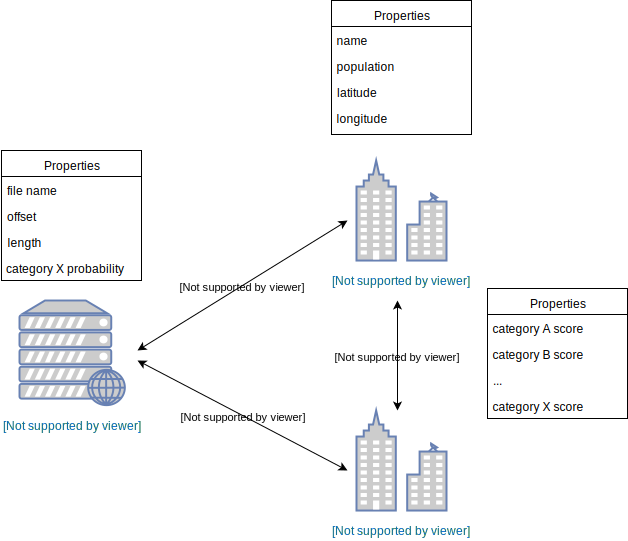
\includegraphics[width=0.6\textwidth]{neo4j-model-full}
    \caption{The Neo4j model as implemented}
    \label{fig:neo4j-model-full}
\end{figure}

During the first tests of the database functions, it appeared that matching and creating was very slow. Checking the query plans (by means of prepending the very useful \texttt{PROFILE} to the queries) gave no hints however. It turned out that we did not use parameterised queries, where we should have. Because of this, Cypher had to recompile, plan and optimise the queries over and over again, which is clearly unnecessary if only the query parameters change. To illustrate the effect of this change, consider the list of cities we used, containing over 1600 cities. Matching all of these in a single transaction by name, without parameterising the query, comes down to repeating the following query for every city:

\begin{lstlisting}[language=cypher, caption={Matching cities without parameterising}, label={lst:query-non-param}]
MATCH (c:City { name: 'Amsterdam' }) RETURN c.name
\end{lstlisting}

The same approach can be used for a parameterised query, where \texttt{\{name\}} is the parameter:
\begin{lstlisting}[language=cypher, caption={Matching cities without parameterising}, label={lst:query-with-param}]
MATCH (c:City { name: {name} }) RETURN c.name
\end{lstlisting}

Even for these 1600 simple matches, the improvements are already significant, as can be seen in table \ref{tbl:param-improvement}.
\begin{table}[H]
\centering
\begin{tabular}{|c|c|}
    \hline
    non-parameterised & 2.84s \\
    parameterised & 0.85s\\
    \hline
\end{tabular}
\caption{Parameterised versus non-parameterised total execution times}
\label{tbl:param-improvement}
\end{table}

Another issue that was encountered during initial testing, is that executing only one query at a time creates and commits a transaction for every query. This is an expensive process. Using the parameterised query from listing \ref{lst:query-with-param} in a single transaction is a 15\% performance gain, as shown in table \ref{tbl:bulk-improvement}. Moreover, it seemed as if performance was fluctuating with a transaction per query. However, we have not bench marked this.
\begin{table}[H]
\centering
\begin{tabular}{|c|c|}
    \hline
    single transaction & 1.07s \\
    parameterised & 0.85s\\
    \hline
\end{tabular}
\caption{Parameterised versus non-parameterised total execution times}
\label{tbl:bulk-improvement}
\end{table}

As will be explained later in section \ref{sec:main-app}, we use multiprocessing to glue the system together efficiently. However, it turned out that Neo4j did not behave correctly when nodes and relations where matched, updated or created from multiple processes. The number of queries performed did not match the number of results returned. In fact, the numbers diverged about 15\%. However, we currently suspect it is not a platform-wide issue. The server the system runs on successfully inserted 154000 \texttt{:Index} labelled nodes and created all required relations, with the use of multiprocessing. We currently suspect (but cannot verify) the problem is related to the version of Neo4j designed for macOS (which half of the group uses). However, we only discovered this close to the deadline of the project. We therefore decided not to include multiprocessing at all for database communication.
